
\begin{figure*}[!t]
\begin{minipage}{.5\linewidth}
\centering
        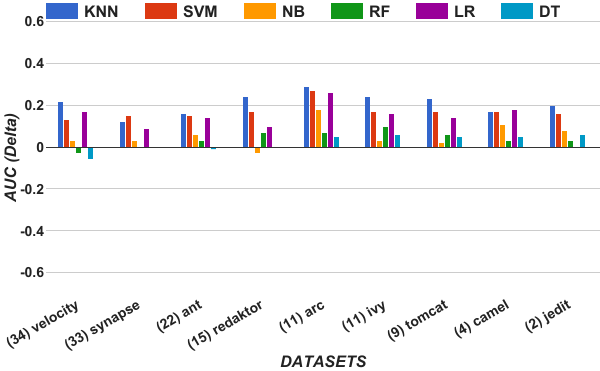
\includegraphics[width=.95\linewidth]{./fig/AUC_untuned.png}
        
  {\bf Figure~\ref{fig:untuned}a:} AUC (pf, recall)
        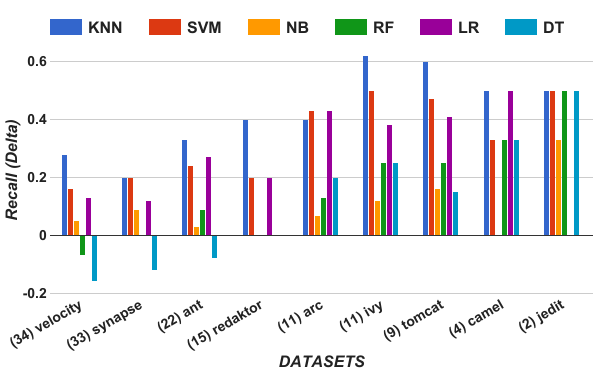
\includegraphics[width=.95\linewidth]{./fig/Recall_untuned.png}
  {\bf Figure~\ref{fig:untuned}c:} Recall
    \end{minipage}%
\begin{minipage}{.5\linewidth}
        \centering
        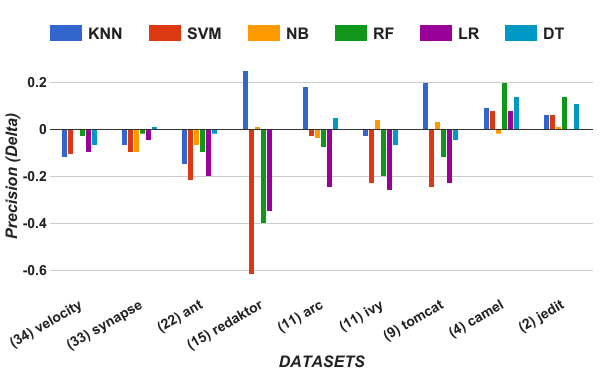
\includegraphics[width=.95\linewidth]{./fig/prec_untuned.png}
  {\bf Figure~\ref{fig:untuned}b:} Precision
        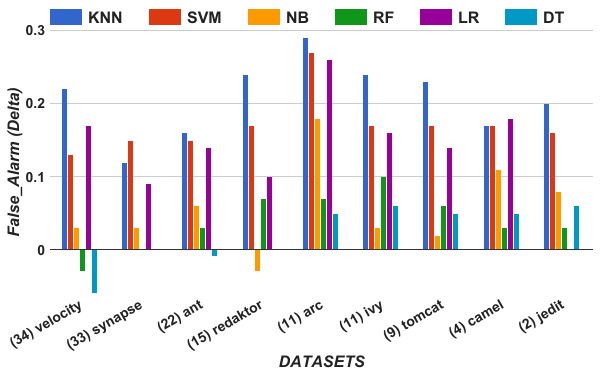
\includegraphics[width=.95\linewidth]{./fig/pf_untuned.png}
  {\bf Figure~\ref{fig:untuned}d:} False Alarm
    \end{minipage}%
    \caption{SMOTE~1 improvement over No SMOTE}
    \label{fig:untuned}
\end{figure*}

\begin{figure*}[!t]
\begin{minipage}{.5\linewidth}
\centering
        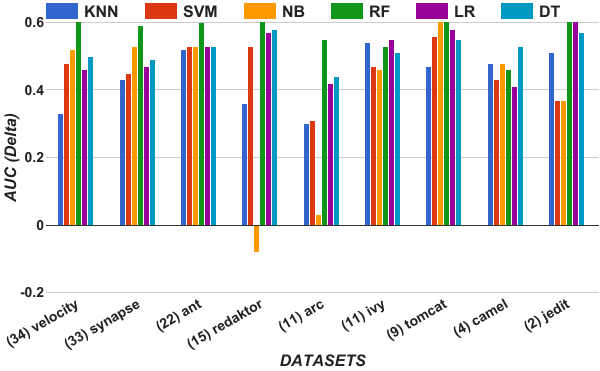
\includegraphics[width=.95\linewidth]{./fig/AUC_tuned.png}
        
  {\bf Figure~\ref{fig:tuned}a:} AUC (pf, recall)
        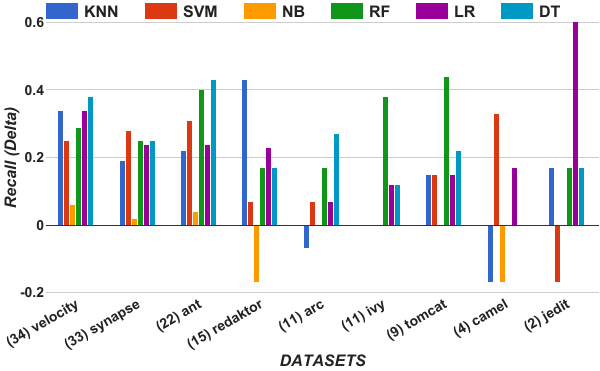
\includegraphics[width=.95\linewidth]{./fig/Recall_tuned.png}
  {\bf Figure~\ref{fig:tuned}c:} Recall
    \end{minipage}%
\begin{minipage}{.5\linewidth}
        \centering
        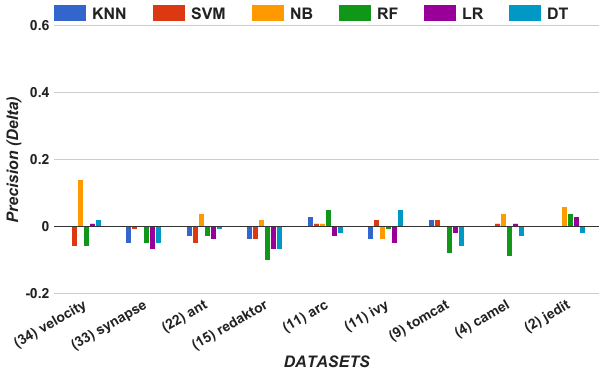
\includegraphics[width=.95\linewidth]{./fig/prec_tuned.png}
  {\bf Figure~\ref{fig:tuned}b:} Precision
        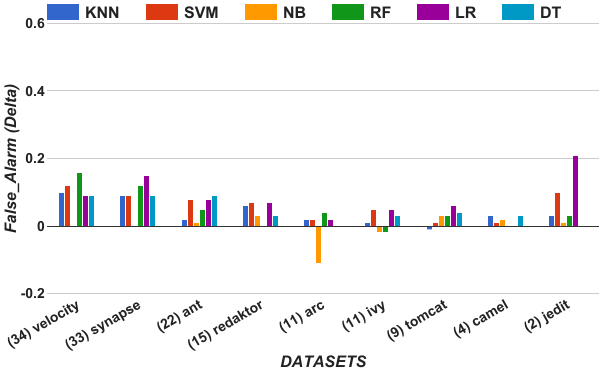
\includegraphics[width=.95\linewidth]{./fig/pf_tuned.png}
  {\bf Figure~\ref{fig:tuned}d:} False Alarm
    \end{minipage}%
    \caption{SMOTE~2 improvement over SMOTE~1}
    \label{fig:tuned}
\end{figure*}

\section{Results}
\label{sect:results}
Figure~\ref{fig:untuned} represents the improvement of SMOTE~1 (median value) against the No SMOTE (median value) results and figure~\ref{fig:tuned} represents the improvement of SMOTE~2 (median value) against SMOTE~1 (median value) results. Each figure contains subfigures to all the 4 evaluation measures (mentioned in \tion{measure}) compared with 6 learners (mentioned in \tion{classes}). X-axis represents all 9 data sets in the decreasing percentage of defective classes from left to right. The corresponding percentage of minority class (in this case, defective class) is written beside each data set. 

For subfigures (AUC, Recall and Precision) in each figure~\ref{fig:untuned} and \ref{fig:tuned}, more positive the better and if it goes negative then the corresponding learners performed worse. On the other hand for subfigure (false alarm), it is other way around. Negative represents better and more positive shows worse results. 

For example of SMOTE~1 improvement over No SMOTE (figure~\ref{fig:untuned}), AUC values are shown in figure~\ref{fig:untuned}a. Redaktor data set is selected from X-axis, and yellow bar represents NB which corresponds to about $-0.05$ AUC value. This denotes that NB performed better without using SMOTE. On the other hand for the same data set, KNN (which is represented in dark blue bar) shows the value of $0.24$. This shows KNN performed way better after applying SMOTE. Now, for NB (still represented by yellow bar), false alarm value (represented in figure~\ref{fig:untuned}d) is about $-0.03$ for the same data set, redaktor. This informs that NB reduces the false positive (FP from figure \ref{fig:cmatrix}) after applying SMOTE. On the other hand for same data set, KNN worsens the false alarm making it to not recommend the use of SMOTE if evaluation goal is false alarm.

For SMOTE~2 improvement over SMOTE~1 (figure~\ref{fig:tuned}), AUC values are shown in subfigure~\ref{fig:tuned}a. Redaktor data set is selected from X-axis, and yellow bar represents NB which corresponds to about $-0.08$ AUC value. This denotes that NB performed worse by tuning the parameters of SMOTE~1. The original parameter settings of SMOTE~1 worked the best. On the other hand for the same data set, KNN (which is represented in dark blue bar) shows the AUC value of $0.35$. This shows KNN outperformed the ``off-the-shelf'' SMOTE~1 when tuned using DE.

\subsection{\textbf{RQ1: Is standard ``off-the-shelf'' SMOTE1 preprocessing method important for defect prediction?}}

By looking at the results of AUC from figure~\ref{fig:untuned}a, only 4 bars are negative, and rest all the remaining 50 bars (in total 9 data sets with 6 learners in each) have  positive effect by using SMOTE~1 as a preprocessing method. We are seeing a maximum improvement of about 30\%. These improvements are quite modest as to ignore the importance of SMOTE.

Results for precision (in figure~\ref{fig:untuned}b), are not much interesting, but the decrease in precision value is not that arduous except for the redaktor data set. Though we will not recommend using SMOTE whenever we want higher precision value. Since precision is decreased using SMOTE, it was expected to have increased false alarm \cite{menzies2007problems} and the same is observed from figure~\ref{fig:untuned}d. There is an increase in error among false positives but the increase is very minimal.

As for recall (figure~\ref{fig:untuned}c), only 4 bars are negative, and rest all the remaining 50 bars (in total 9 data sets with 6 learners in each) have positive effect by using SMOTE~1. We are seeing a maximum improvement of about 60\%. These improvements are quite steep as to ignore the importance of SMOTE at any point for any learner. It is also observed that performance keeps increasing as target class becomes more minor and minor. This is what was expected after applying SMOTE to imbalance data sets.

\begin{lesson1}
    For defect data, SMOTE1 has little added value for 
 precision, modest improvements for AUC (pf,recall) and largest improvements for recall.
\end{lesson1}

\subsection{\textbf{RQ2: Can tuning SMOTE~1 (SMOTE~2) achieve better results?}}

Now when we look at the results of AUC from figure~\ref{fig:tuned}a, only 1 bar is negative, and rest all the remaining 53 bars (in total 9 data sets with 6 learners in each) have  positive effect after when we tune the parameters of SMOTE~1. We are seeing a maximum improvement of about 70\% and on an average 50\% for each learner in all data sets. These improvements are quite steep in nature and just to remind you that these results are improvement over SMOTE~1. If we combine the results, then we can surely say to tune the parameters of SMOTE~1 and train using any learner, we will get atleast 100\% improvement in most cases.

We are seeing the similar trend of results for precision (in figure~\ref{fig:tuned}b), just like in Figure~\ref{fig:untuned}b, that even after tuning for precision, we are not seeing much improvement. Though we definitely improved precision slightly than SMOTE~1 but the increment is not that large to recommend SMOTE~2 or SMOTE~1. And even after trying to minimise the false alarm (figure~\ref{fig:tuned}d) value, DE could not find a good parameter setting.

As for recall (figure~\ref{fig:untuned}c), only 5 bars are negative, and rest all the remaining 49 bars (in total 9 data sets with 6 learners in each) have either positive effect or no effect after tuning. We are seeing a maximum improvement of about 65\% but the average improvement is close to 15\% for each classifiers in all data sets. But these improvements combined with SMOTE~1 suggest that we should always tune SMOTE~1 whenever the goal is to achieve higher recall.

\begin{lesson1}
    For defect data, SMOTE2  
 offers   large  improvements over SMOTE1 for recall
 and dramatic improvements for AUC (pf, recall).
\end{lesson1}

\begin{figure*}[!t]
    \centering
    \begin{minipage}{.33\textwidth}
        \captionsetup{justification=centering,singlelinecheck=off}
        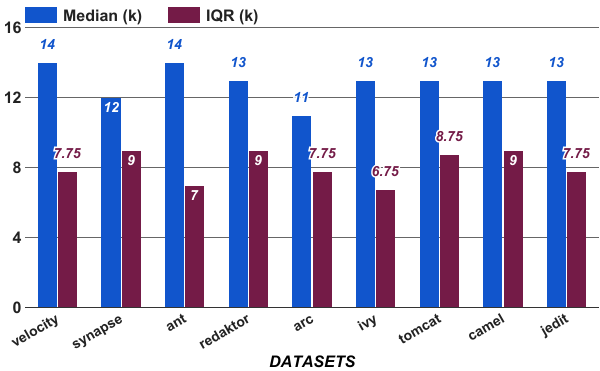
\includegraphics[width=.95\linewidth]{./fig/k.png}
        \caption{Data sets vs Parameter ($k$) variation}
        \label{RQ3:k}
    \end{minipage}%
    \begin{minipage}{.33\textwidth}
        \captionsetup{labelsep=space,justification=centering,singlelinecheck=off}
        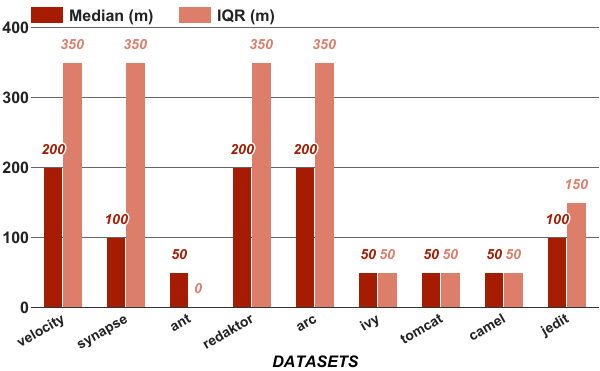
\includegraphics[width=.95\linewidth]{./fig/m.png}
        \caption{Data sets vs Parameter ($m$) variation}
        \label{RQ3:a}
    \end{minipage}
    \begin{minipage}{.33\textwidth}
        \captionsetup{labelsep=space,justification=centering,singlelinecheck=off}
        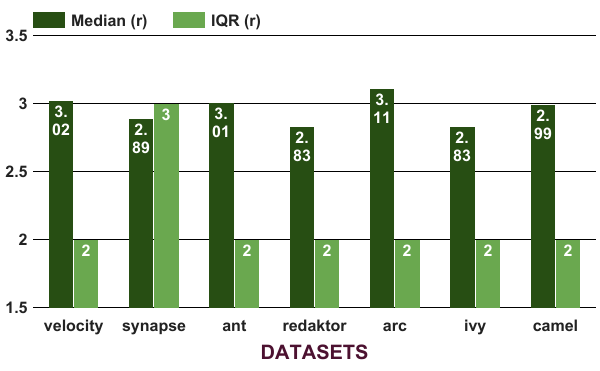
\includegraphics[width=.95\linewidth]{./fig/r.png}
        \caption{Data sets vs Parameter ($r$) variation}
        \label{RQ3:b}
    \end{minipage}
\end{figure*}

\subsection{\textbf{RQ3: Do different data sets
      need different configurations with SMOTE2?}}

Figures \ref{RQ3:k}, \ref{RQ3:a}, and \ref{RQ3:b} show the results of tuning for each data set when recall is considered as evaluation goal. These parameter settings are found by each learner for that data set.
On display in each set of vertical bars are
the median values generated across 15 evaluations.
Also, shown are
the inter-quartile range (IQR) of those tunings (the IQR is the 75th-25th percentile values and is a non-parametric measure of variation
around the median value). Note that in Figure \ref{RQ3:a}, IQR=0 for  ant data set where tuning
          always converged on the same final value.

  These figures
show how tuning selects the different ranges  of
parameters. 
Some of the above numbers are far from the standard values; e.g. Chawla et al.~\cite{chawla2002smote} recommend using $k=$5 neighbors yet in our data sets, best results were seen using $k \approx 13$. On other hand it was suggested to use $m=900$ by ~\cite{pears2014synthetic}, but best results vary with each data set.

Clearly:
\begin{lesson1}
    DE finds different ``best'' parameter settings for SMOTE for different data sets. Hence reusing tunings  suggested  by  any other  previous study  for any data set is \underline{{\em not}} recommended. Instead,  it is better to
      use  automatic  tuning  methods  to find the best tuning parameters for the current data set.
\end{lesson1}

\begin{figure}[!b]
  \captionsetup{justification=centering}
  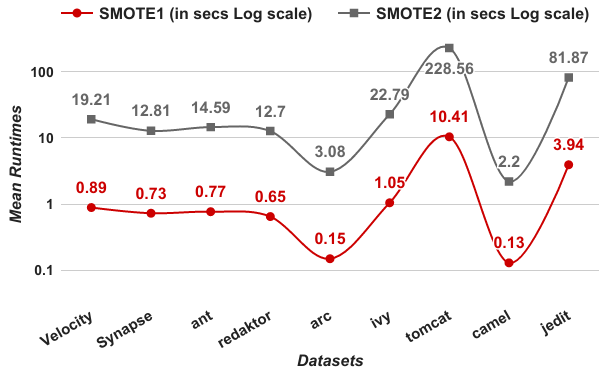
\includegraphics[width=\linewidth]{./fig/runtimes.png}
  \caption{Data sets vs Runtimes}
  \label{runtime}
\end{figure} 

\subsection{\textbf{RQ4: Is tuning extremely slow?}}

Search-based SE methods can be very slow. Wang et al.~\cite{wang2013searching} once needed 15
years of CPU time to find and verify the tunings required for software
clone detectors. Sayyad et al.~\cite{sayyad2013scalable} routinely used
$10^6$ evaluations (or more) of their models in order to extract
products from highly constrained product
lines. Hence, before recommending any
search-based method, it is wise to consider the runtime cost of that
recommendation.

To understand our timing results, recall that SMOTE2 uses
Algorithm~1. Based on the psuedocode
shown above, our pre-experimental expectation is that
tuning will be three to fives times slower than not tuning. Figure~\ref{runtime} has runtimes for 1 tuning goal with 1 learner in question.
 
Figure~\ref{runtime} check if that theoretical
holds true in practice. Shown in circle and square markers are the
  runtimes required to run SMOTE1 and SMOTE2 respectively.  The
  longer runtimes (in square) include the times required for DE to find
  the tunings. Overall, tuning slows down the training by a factor of up to
  five (which is very close to our theoretical prediction).

\begin{lesson1}
    Tuning with DE makes training four to five times slower, but the improvements which we get for AUC and recall is quite advantageous.
\end{lesson1}
